\section{Sparse Identification of Nonlinear Dynamical Systems}

Extracting the governing equations from data has been a great challenge in the fields of science and engineering.
While recent rapid advances in machine learning and data science have enabled the ability to analyze and understand complex static data, methods for capturing physical models of dynamical systems from data have slowly progressed.
To ease this problem, the \gls{SINDy} method was proposed for discovering the underlying dynamics of systems using sparse regression and compressed sensing \cite{bruntonDiscoveringGoverningEquations2016}.
Given the dynamical systems of the form
\begin{equation}
    \frac{d}{dt} x(t) = f(x(t)),
\end{equation}
where $x(t)$ is a vector of the state of the system at time $t$, and the function $f(x(t))$ describes the dynamic constraints that define the behaviors of the system.
One key observation made by the author is that in many dynamical systems, the governing function $f$ is sparse in the space of possible functions.
Under that observation, methods in compressed sensing and sparse regression can be used to determine which terms are most likely to describe $f$ without performing a brute-force search \cite{bruntonDiscoveringGoverningEquations2016}.

\begin{figure}[h]
    \centering
    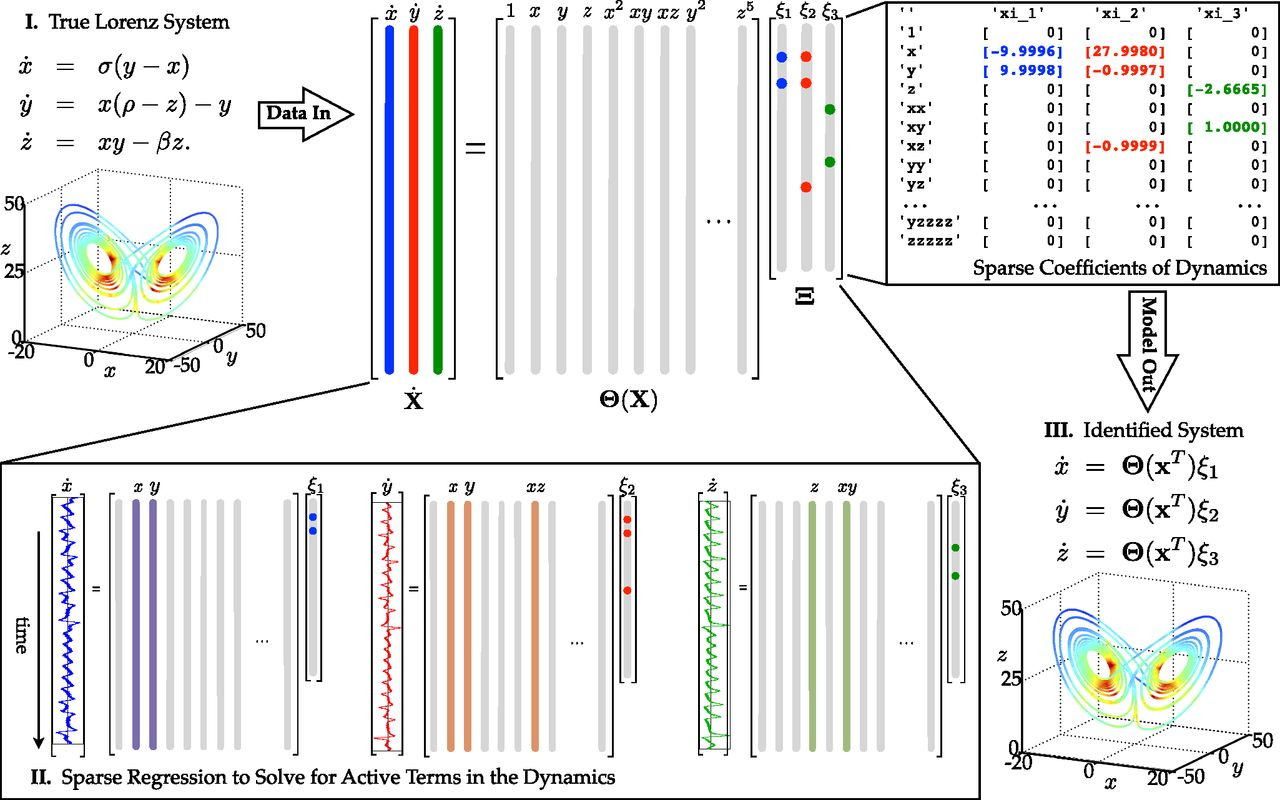
\includegraphics[scale=1.4]{sindy-schematic.png}
    \caption{Schematic of the SINDy algorithm, demonstrated on the Lorenz equations. The few entries in the vectors of $\Xi$, solved for by sparse regression, denote the relevant terms in the right-hand side of the dynamics. Parameter values are $\sigma = 10$, $\beta = 8/3$, $\rho = 28$, $(x_0 , y_0 , z_0)^T = (-8,7,27)^T$. The trajectory on the Lorenz attractor is colored by the adaptive time step required, with red indicating a smaller time step. Figure is taken from \cite{bruntonDiscoveringGoverningEquations2016}}
    \label{fig:sindy-schematic}
\end{figure}

To determine the function $f$ from data, the history of the state $x(t)$ and its derivative $\dot{x}(t)$ at time step $t_1, t_2, \cdots, t_m$ are collected \cite{bruntonDiscoveringGoverningEquations2016}
\begin{equation}
    \begin{aligned}
        X &=
        \begin{bmatrix}
            X^T(t_1) \\
            X^T(t_2) \\
            \vdots \\
            X^T(t_m)
        \end{bmatrix} =
        \begin{bmatrix}
            x_1(t_1) & x_2(t_1) & \cdots & x_n(t_1) \\
            x_1(t_2) & x_2(t_2) & \cdots & x_n(t_2) \\
            \vdots & \vdots & \ddots & \vdots \\
            x_1(t_m) & x_2(t_m) & \cdots & x_n(t_m)
        \end{bmatrix}, \\
        \dot{X} &=
        \begin{bmatrix}
            \dot{X}^T(t_1) \\
            \dot{X}^T(t_2) \\
            \vdots \\
            \dot{X}^T(t_m)
        \end{bmatrix} =
        \begin{bmatrix}
            \dot{x}_1(t_1) & \dot{x}_2(t_1) & \cdots & \dot{x}_n(t_1) \\
            \dot{x}_1(t_2) & \dot{x}_2(t_2) & \cdots & \dot{x}_n(t_2) \\
            \vdots & \vdots & \ddots & \vdots \\
            \dot{x}_1(t_m) & \dot{x}_2(t_m) & \cdots & \dot{x}_n(t_m)
        \end{bmatrix}.
    \end{aligned}
\end{equation}
Next, a library $\Theta(X)$ of candidate nonlinear functions of the columns of $X$ is constructed.
An example of a library that consists of constant, polynomial, and trigonometric terms is given \cite{bruntonDiscoveringGoverningEquations2016}
\begin{equation}
    \Theta(X) = \begin{bmatrix}
        | & | & |       & |       &        & |      & |      & \\
        1 & X & X^{P_2} & X^{P_3} & \cdots & sin(X) & cos(X) & \cdots \\
        | & | & |       & |       &        & |      & |      &
    \end{bmatrix},
\end{equation}
where $X^{P_n}$ denotes higher polynomials, i.e., $X^{P_2}$ denotes quadratic nonlinearities in the state $x$
\begin{equation}
    X^{P_2} = \begin{bmatrix}
        x_1^2(t_1) & x_1(t_1)x_2(t_1) & \cdots & x_2^2(t_1) & \cdots & x_n^2(t_1) \\
        x_1^2(t_2) & x_1(t_2)x_2(t_2) & \cdots & x_2^2(t_2) & \cdots & x_n^2(t_2) \\
        \vdots     & \vdots           & \ddots & \vdots     & \ddots & \vdots \\
        x_1^2(t_n) & x_1(t_n)x_2(t_n) & \cdots & x_2^2(t_n) & \cdots & x_n^2(t_n)
    \end{bmatrix}.
\end{equation}
Each column of $\Theta(X)$ represents a candidate function for the dynamics $f(x(t))$.
Based on the observation on the sparsity of terms, i.e., only a few of the nonlinearities are active, a sparse regression problem can be set up to determine the vector of coefficients $\Xi = [\xi_1\ \xi_2\ \cdots\ \xi_n]$ such that \cite{bruntonDiscoveringGoverningEquations2016}
\begin{equation}
    \dot{X} = \Theta(X)\Xi.
\end{equation}
Once $\Xi$ has been found, the governing equations can be constructed as \cite{bruntonDiscoveringGoverningEquations2016}
\begin{equation}
    \dot{x} = f(x) = \Xi^T(\Theta(X^T))^T,
\end{equation}
where $\Theta(X^T)$ is a vector of symbolic functions of $x$, unlike $\Theta(X)$ which is a data matrix.

The effectiveness of the \gls{SINDy} method depends on the choice of measurements, data quality, and sparsity of the function basis.
In some problems, the columns of $\Theta(X)$ might need to be normalized, particularly when entries in $X$ are small.
One might need to test with different bases and use the sparsity and accuracy as evaluation metrics for the resulting model.
In many areas, the data for the derivative $\dot{X}$ of $X$ can not be measured, and $\dot{X}$ has to be numerically approximated which introduces noise into the data.
These noises make it hard to find the true governing equations of the system.
The \gls{SINDy} method is also ill-suited for problems with a high state dimension, where dimensionality reduction techniques can not be applied.
In general, the right coordinates and function basis are needed to yield correct sparse dynamics.
Requirements on the system and solutions for overcoming these shortcomings are discussed in detail in the original paper \cite{bruntonDiscoveringGoverningEquations2016}.